
\section{Development Process}
\label{sec:taxonomy_development_process}

\begin{figure}[t]
    \centering
    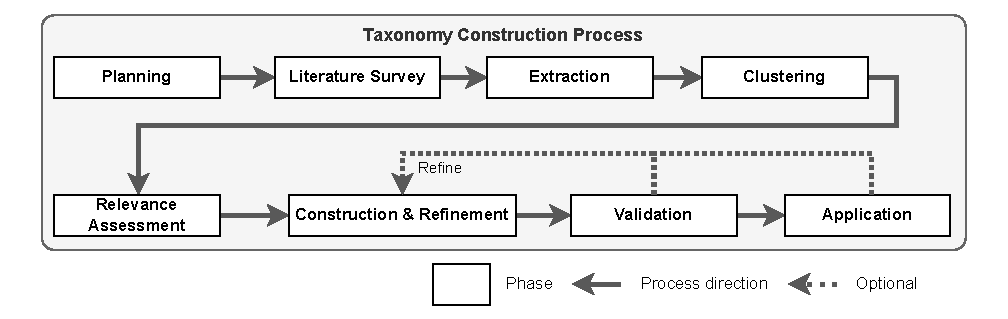
\includegraphics[width=0.99\linewidth]{figures/question_catalog/taxonomy-construction_process_general.drawio.pdf}
    \caption[Taxonomy Construction Process]{The taxonomy construction process involving eight consecutive phases to synthesize knowledge from the literature into a taxonomy that is then incrementally refined and validated.}
    \label{fig:taxonomy_development_process}
\end{figure}

The overall development process is illustrated in \autoref{fig:taxonomy_development_process}. It consists of eight consecutive phases. The process begins with the \textsc{Planning} phase, where the intended use of the taxonomy is defined. In the following \textsc{Literature Survey} phase, a literature review is conducted to collect potential candidates that contain relevant terms, which we refer to as classes. These candidates are then manually extracted in the \textsc{Extraction} phase to identify the relevant classes from the text. In the \textsc{Clustering} phase, the extracted classes are merged in a deduplication process and subsequently grouped into semantic categories. These categories are then evaluated for their relevance in the \textsc{Relevance Assessment} phase. The remaining categories are used to initialize the first taxonomy increment during the \textsc{Construction and Refinement} phase. This increment is then evaluated in the \textsc{Validation} phase to determine whether revisions are necessary. If so, the process returns to the previous phase. Otherwise, it proceeds to the \textsc{Application} phase, where the practical use of the taxonomy is demonstrated in a specific application scenario. In the following sections, we take a closer look at each phase of the process.


\subsection{Planning}
\label{sec:tax_dev_planning}

The first phase of the process is \textsc{Planning}. In this phase, the objective and intended use of the taxonomy is defined. Additionally, characteristics of the taxonomy that should be considered during its development are specified.

According to \textcite{usman_taxonomies_2017}, six activities should be carried out when planning a taxonomy. However, it is important to note that the authors focused specifically on the software engineering domain. For our process, we aim to maintain general applicability. Therefore, we have adapted these activities and formulated the following steps for the \textsc{Planning} phase:


\begin{enumerate}[label=\textbf{S\arabic*:}, leftmargin=2.5em]
    \item \label{enum:step1} Define one or more declarative sentences that clearly define the objective and scope of the taxonomy.
    \item \label{enum:step2} Define the domain for which the taxonomy is to be applied.
    \item \label{enum:step3} Define the structure type of the taxonomy.
    \item \label{enum:step4} Define the procedure type of the taxonomy.
    \item \label{enum:step5} Define the topics and domains of the literature from which the collection of classes takes place.
\end{enumerate}

In the first step, \textbf{S1}, the goal of the taxonomy should be clearly defined so that users understand the use cases it is meant to support. To achieve this, one or more declarative sentences should be formulated that narrow the scope and clearly express the intended purpose. 

Step \textbf{S2} involves defining the domain of the taxonomy. This should help users assess whether the taxonomy is intended for a specific domain and allow them to better understand its scope.

In \textbf{S3}, the structure of the taxonomy is specified. According to \textcite{usman_taxonomies_2017}, there are four different types of structures, which we will explain briefly. A taxonomy with a \emph{hierarchy} structure has a single parent class that contains multiple subclasses. In contrast, a \emph{tree} structure does not imply inheritance relationships between classes. Instead, it features a parent class with subclasses that can represent relationships such as part-whole, cause-effect, and process-product. A \emph{paradigm} taxonomy represents a two-dimensional matrix classification, where each cell represents a combination of possible classes. Finally, a \emph{faceted} taxonomy captures multiple independent perspectives or \enquote{facets}, each with its own set of classes.

In step \textbf{S4}, the procedural type of the taxonomy has to be defined. This procedure describes how instances are systematically assigned to the classes or categories of the taxonomy. The procedure depends on the measurement method used for the classification and is divided into two types, according to \textcite{usman_taxonomies_2017}. \emph{Qualitative} procedures use nominal scales, which means that the classification is based on descriptive attributes. \emph{Quantitative} procedures, on the other hand, use numerical scales for classification.

The final step in the planning phase is \textbf{S5}, which involves categorizing the literature from which the classes will be extracted according to their topics and domains. This helps users understand the data foundation from which the taxonomy has been derived.

\subsection{Literature Survey}
\label{sec:tax_con_literature_survey}

The second phase of the development process is named \textsc{Literature Survey}. The goal is to identify candidates from the literature that potentially contain relevant classes for the taxonomy. The survey is conducted iteratively, with transparency and repeatability serving as top priorities. Furthermore, this iterative approach allows the process to be paused early if needed and resumed at a later time. 

Two lists are defined to conduct the literature survey: \emph{Intermediate List} and \emph{Final List}. The intermediate list is defined for each iteration and is denoted as $\mathcal{L}_i$, where $i \in \mathbb{N}_{>0}$ indicates the current iteration. This list contains all the literature resources that have been processed during that specific iteration. This processing is done using the \hyperref[enum:processing_paper_task]{\textbf{Processing Paper Task}} described below. During this task, new candidates may be extracted from a resource $\mathcal{P}$, which then forms the list for the next iteration, $\mathcal{L}_{i+1}$, such that:

\[
\mathcal{L}_{i+1} = \bigcup_{\mathcal{P} \in \mathcal{L}_i} \left( \text{Ref}(\mathcal{P}) \cup \text{CitedBy}_n(\mathcal{P}) \right)
\]

Here, $\text{Ref}(\mathcal{P})$ refers to the set of relevant references from the bibliography of $\mathcal{P}$, while $\text{CitedBy}_n(\mathcal{P})$ represents the first $n$ publications assessed as relevant from a \emph{Cited by} search. 

In addition, the literature survey process has a second list named \emph{final list} which is denoted as $\mathcal{F}$. This list contains all literature resources that have been assessed as relevant in any of the conducted iterations of the process.

The following section illustrates the literature survey process, which is based on the guidelines for conducting a systematic literature review by \textcite{wohlin_guidelines_2014}:


\paragraph{Literature Survey Process}
\begin{enumerate}
    \item \textbf{Prepare Seeds:} Collect seed papers and add them to $\mathcal{L}_1$.
    \item \textbf{First Iteration:} Process each paper in $\mathcal{L}_1$ by applying the \emph{Processing Paper Task} described below.
    \item \textbf{Additional Search:} Conduct a search e.g. on Google Scholar to find additional papers that are not covered by the seed papers. Add these papers to $\mathcal{L}_2$.
    \item \textbf{More Iterations:} Process each paper in the intermediate list of the current iteration $i \in \mathbb{N}_{>0}$ by applying the \emph{Processing Paper Task} described below. Continue processing until satisfied or there are no more paper candidates in $\mathcal{L}_i$.
\end{enumerate}

\paragraph{Processing Paper Task}
\label{enum:processing_paper_task}
\begin{enumerate}
    \item Collect paper $\mathcal{P}$ from $\mathcal{L}_i$ that has not yet been processed.
    \item Determine whether $\mathcal{P}$ is relevant on the basis of the title and abstract. This is done by applying the defined \emph{inclusion} and \emph{exclusion} criteria. If not relevant, $\mathcal{P}$ is skipped.
    \item The text of $\mathcal{P}$ is skimmed to identify relevant text sections. If no relevant text sections are found, $\mathcal{P}$ is skipped.
    \item If $\mathcal{P}$ is found to be relevant, it is added to the list $\mathcal{F}$.
    \item The reference list of $\mathcal{P}$ is processed to identify possible relevant publications based on their title. Add these candidates to the $\mathcal{L}_{i+1}$.
    \item Using a search engine like Google Scholar, the \emph{cited by} feature is used on $\mathcal{P}$ to collect a list of publications $\hat{\mathcal{C}}$ referencing $\mathcal{P}$. The list is obtained by sorting by relevance and collecting the first $n$ publications. For each $\hat{\mathcal{c}} \in\hat{\mathcal{C}}$, their titles and abstracts are analyzed to consider whether the defined \emph{inclusion} and \emph{exclusion} criteria are met. If so, the paper $\hat{\mathcal{c}}$ is added to $\mathcal{L}_{i+1}$.
\end{enumerate}

To help categorize publications as relevant, inclusion and exclusion criteria should be defined. The exact criteria used depend on the respective objective and domain of the taxonomy.

\subsection{Extraction}

The result of the literature search is the set $\mathcal{F}$, which includes all publications that were classified as relevant. In the \textsc{Extraction} phase, each publication $f \in \mathcal{F}$ is processed by identifying classes for the taxonomy based on the content of the publication. For each relevant publication $f$, a subset $\mathcal{C}_{f}$ is defined, containing all classes extracted from $f$. Each class consists of a name and a description, both taken directly from the respective publication.

The complete set of all extracted classes is defined as the union of all $\mathcal{C}_{f}$ for every $f \in \mathcal{F}$:

\[
\mathcal{C} = \bigcup_{f \in \mathcal{F}} \mathcal{C}_{f}
\]


\subsection{Clustering}
\label{sec:tax_proc_clustering}

The next phase is called \textsc{Clustering} and consists of two main steps. First, the classes $\mathcal{C}$ extracted from the literature are grouped to merge semantically redundant entries. Then, these consolidated classes are organized into categories.

\paragraph{Deduplication}
In the first step, the extracted classes $\mathcal{C}$ are clustered based on their semantic similarity. Classes that are considered equivalent or very similar in meaning, based on their names or descriptions, are grouped together. The level of abstraction at which this merging occurs depends on the specific use case.

Each resulting cluster contains classes that are either semantically equivalent or closely related. The set of these clusters is denoted by $\hat{\mathcal{C}} = {\hat{c}_1, \hat{c}_2, \dots, \hat{c}_n}$, where each cluster $\hat{c}_i$ is a subset of the original class set $\mathcal{C}$, and all clusters are mutually disjoint:

\[
\forall i \ne j: \hat{c}_i \cap \hat{c}_j = \emptyset
\quad \text{and} \quad \bigcup_{i=1}^{n} \hat{c}_i = \mathcal{C}
\]

For each cluster $\hat{c}_i$, a representative class is defined, which provides the cluster with a name and description. This can be done either by selecting an existing class within the cluster or by manually synthesizing a new one based on the contained classes.

\paragraph{Categorization}
In the second step, the class clusters $\hat{\mathcal{C}}$ are grouped into semantically coherent categories, denoted as $\mathcal{K}$. Depending on the context, it may be assumed that these categories are disjoint. Each category $k \in \mathcal{K}$ is assigned a name $n_k$ and a description $d_k$. Naming is based on the interpretation of the deduplicated classes contained in $\hat{C}_k$, with the aim of capturing the overarching semantic context of the included concepts. The description $d_k$ provides clarification and contextual background for the category. A category can thus be represented as a tuple:

\[
k = (\hat{C}_k, n_k, d_k)
\]

Here, $\hat{C}_k \subseteq \hat{\mathcal{C}}$ is the associated group of deduplicated classes, $n_k$ is the name of the category, and $d_k$ is the corresponding description. The complete set of categories is then:

\[
\mathcal{K} = \left\{ (\hat{C}_k, n_k, d_k) \;\middle|\; \hat{C}_k \subseteq \hat{\mathcal{C}} \right\}
\]

\subsection{Relevance Assessment}

During the \textsc{Relevance Assessment} phase, the goal is to evaluate the set of categories $\mathcal{K}$ and their corresponding deduplicated classes $\hat{C}_k$ in terms of their relevance to the target taxonomy. This step reduces the overall set $\mathcal{K}$ to only the categories and classes that are truly significant.

To assess relevance, an evaluation function is defined based on a specified set of qualitative criteria. Each category and class are manually evaluated through content analysis and reasoned judgment. The evaluation function is formalized as follows:

\[
\text{rel}: \hat{\mathcal{C}} \cup \mathcal{K} \rightarrow \{0, 1\}
\]

Where: 
\begin{enumerate} 
    \item $\text{rel}(x) = 1$ if the element $x \in \hat{\mathcal{C}} \cup \mathcal{K}$ is considered relevant, 
    \item $\text{rel}(x) = 0$ otherwise. 
\end{enumerate}

Based on this evaluation function, the sets of relevant classes and categories are defined as follows:

\[
\mathcal{C}^\ast = \{ \hat{c} \in \hat{\mathcal{C}} \mid \text{rel}(\hat{c}) = 1 \}
\quad \text{and} \quad
\mathcal{K}^\ast = \{ k \in \mathcal{K} \mid \text{rel}(k) = 1 \}
\]

Furthermore, if a category $k \in \mathcal{K}$ is evaluated as not relevant, then all its associated classes $\hat{\mathcal{C}}_k \subseteq \hat{\mathcal{C}}$ are also classified as not relevant. Conversely, if a category does not contain any relevant classes, it can be excluded from $\mathcal{K}^\ast$.

 
\subsection{Taxonomy Construction and Refinement}

The phase \textsc{Taxonomy Construction and Refinement} may be carried out multiple times throughout the development process. The goal is to construct a taxonomy based on the categories and classes identified during the \textsc{Relevance Assessment} phase and to refine it iteratively as needed. Each taxonomy increment is denoted by $\mathcal{T}_i$, where $i \in \mathbb{N}{>0}$. The first execution of this phase creates the initial increment $\mathcal{T}_1$. With each subsequent execution, the current increment $\mathcal{T}_i$ is revised to generate an improved increment $\mathcal{T}_{i+1}$.

\paragraph{Taxonomy Initialization} To initialize the taxonomy, the set of categories rated relevant ($\mathcal{K}^\ast$) is used. This set forms the basis for the first taxonomy increment $\mathcal{T}_1$, which describes the structure and content of the taxonomy in its initial version:

\[
\mathcal{T}_1 := \mathcal{K}^\ast
\]

\paragraph{Taxonomy Refinement} If it is determined during the \textsc{Validation} phase that the current increment $\mathcal{T}_i$ has weaknesses in terms of generality, appropriateness, orthogonality, or novelty, a targeted refinement step is carried out to address them. During this step, individual categories or classes may be created, adjusted, moved, merged, or removed. The result is a new increment $\mathcal{T}_{i+1}$, derived from a modified version of $\mathcal{T}_i$:

\[
\mathcal{T}_{i+1} = \text{Refine}(\mathcal{T}_i, \Delta_i)
\]

Here, $\Delta_i$ represents the set of all change operations identified during the refinement.

\subsection{Validation}

In the \textsc{Validation} phase, the current increment of the taxonomy $\mathcal{T}_i$ is evaluated based on the criteria \emph{Generality}, \emph{Appropriateness}, \emph{Orthogonality}, and \emph{Novelty}. For this validation, the goals \textbf{G1} and \textbf{G2} from the \gls{gqm} plan are taken into account, which are outlined in \autoref{tab:gqm_taxonomy_validation}.

Various metrics are used for validation, each having the form $f(\alpha, \beta)$. Here, $\alpha$ represents the set of classes from the current taxonomy, while $\beta$ denotes the comparison set. In this context, $\mathcal{K}_{\mathcal{T}_i}$ refers to the categories of the current taxonomy, $\mathcal{C}_k$ to the not yet deduplicated classes within a category $k \in \mathcal{K}_{\mathcal{T}_i}$, and $\mathcal{C}_{\mathcal{T}_i}$ to the complete set of classes in $\mathcal{T}_i$:

\[
\mathcal{C}_{\mathcal{T}_i} = \bigcup_{k \in \mathcal{K}_{\mathcal{T}_i}} \mathcal{C}_k
\]

As previously defined, $\mathcal{C}$ represents the set of all classes extracted from the literature. The metrics are thus applied as $f(\mathcal{C}_{\mathcal{T}_i}, \mathcal{C})$, comparing the classes in the current taxonomy with the extracted set. Note that we refer to the classes before the deduplication process here. The validation is then carried out by answering the following questions according to the \gls{gqm} plan:

\paragraph{Generality and Granularity} Question \hyperref[tab:gqm_taxonomy_validation]{\textbf{Q1.1}} investigates whether the taxonomy demonstrates an appropriate level of generality and granularity. The metrics \emph{Laconicity} (\hyperref[tab:gqm_taxonomy_validation]{\textbf{M1.1.1}}) and \emph{Lucidity} (\hyperref[tab:gqm_taxonomy_validation]{\textbf{M1.1.2}}) are used for this evaluation. A high \emph{Laconicity} score is expected in the first increment $\mathcal{T}_1$, since the initialization is based directly on the classes from the literature. In contrast, a low \emph{Lucidity} score can be desirable depending on the context, as it indicates that many classes in the taxonomy are supported by multiple sources in the literature, which reflects broad acceptance.

\paragraph{Appropriateness} Question \hyperref[tab:gqm_taxonomy_validation]{\textbf{Q1.2}} assesses whether the content of the taxonomy is suitable for its intended purpose. The supporting metrics are \emph{Completeness} (\hyperref[tab:gqm_taxonomy_validation]{\textbf{M1.2.1}}) and \emph{Soundness} (\hyperref[tab:gqm_taxonomy_validation]{\textbf{M1.2.2}}). A high \emph{Completeness} score indicates that a large proportion of the extracted classes $\mathcal{C}$ are present in $\mathcal{T}_i$. In contrast, \emph{Soundness} is at its maximum in the first increment $\mathcal{T}_1$, since all included classes at that stage are derived from the literature: $\mathcal{C}_{\mathcal{T}_1} \subseteq \mathcal{C}$.

\paragraph{Orthogonality} Question \hyperref[tab:gqm_taxonomy_validation]{\textbf{Q1.3}} examines potential overlaps between classes of different categories within $\mathcal{T}_i$. An orthogonality matrix (\hyperref[tab:gqm_taxonomy_validation]{\textbf{M1.3.1}}) is created to make these overlaps visible.

\paragraph{Relevance} Question \hyperref[tab:gqm_taxonomy_validation]{\textbf{Q2.1}} checks whether the classes included in the taxonomy are actually relevant to the intended purpose. The evaluation is based on a qualitative analysis for each class. After the relevance for each class has been asserted, a total relevance score (\hyperref[tab:gqm_taxonomy_validation]{\textbf{M2.1.1}}) is calculated. Since the initial taxonomy $\mathcal{T}_1$ is based on the pre-filtered set $\mathcal{K}^\ast$, a high level of relevance is already ensured. If new classes are added in later increments, their relevance must be discussed explicitly.

\paragraph{Novelty} Question \hyperref[tab:gqm_taxonomy_validation]{\textbf{Q2.2}} addresses the degree of innovation in the taxonomy. It explores whether a meaningful number of new categories or classes have been introduced. The evaluation is based on the metrics \hyperref[tab:gqm_taxonomy_validation]{\textbf{M2.2.1}} (\emph{Innovation}) and \hyperref[tab:gqm_taxonomy_validation]{\textbf{M2.2.2}} (\emph{Adoption}). For the first increment $\mathcal{T}_1$, a minimal value is expected, as no new concepts have been introduced beyond those collected in $\hat{\mathcal{C}}$.

If discrepancies are identified during validation, the process returns to the \textsc{Taxonomy Construction and Refinement} phase to create a new taxonomy increment $\mathcal{T}_{i+1}$ to resolve these issues.



\subsection{Application}

Once the \textsc{Validation} phase has confirmed that a taxonomy increment $\mathcal{T}_i$ meets the required quality standards, the process continues with the \textsc{Application} phase. The purpose of this phase is to demonstrate the applicability and usefulness of the taxonomy in specific scenarios.

To accomplish this, the final increment $\mathcal{T}_i$ is applied to selected use cases. This involves assigning concrete questions, objects, or entities to the categories and classes of the taxonomy. If issues arise during this process, such as missing, unclear, or unsuitable categories or classes, the development returns to the \textsc{Taxonomy Construction and Refinement} phase. In this case, a new increment $\mathcal{T}_{i+1}$ is created to address the identified issues. Therefore, the \textsc{Application} phase not only serves to demonstrate the practical utility of the taxonomy but also acts as a final validation loop in the form of a controlled real-world test.

The application phase is further supported by question \hyperref[tab:gqm_taxonomy_validation]{\textbf{Q2.3}}, which is evaluated using the metric \emph{Classification Delta} (\hyperref[tab:gqm_taxonomy_validation]{\textbf{M2.3.1}}). The goal is to determine the significance of the taxonomy in terms of its actual classification performance. Formally, let $\mathcal{U}$ be a set of use cases to be tested, and let $\hat{\mathcal{T}}$ be a comparison set of alternative taxonomies. The metric calculates the classification difference as follows:
\[
\Delta(\mathcal{U}, \mathcal{T}_i, \hat{\mathcal{T}}) = f_{\text{delta}}(\mathcal{U}, \mathcal{T}_i, \hat{\mathcal{T}})
\]

The higher the value of $\Delta$, the more significant the evaluated taxonomy is compared to the alternatives. However, the acceptable level of significance depends on the specific use case and must be interpreted appropriately within the domain-specific context.

% Each step in the process of developing the taxonomy also produced several research artifacts which thoroughly document the whole development process. These artifacts have been carefully designed and planned to allow for high reproducibility of the development process. This is made possible through defining well-formed JSON files, where the information for each step is structured to allow for an easy 1) machine readability and 2) manual modification or extension. This machine readability is then utilized in several PYTHON scripts, where the data is automatically extracted from the structured data in the JSON files to perform analyses. In case that the development process is repeated or extended, the above-mentioned procedure allows us to reproduce or modify the taxonomy with further data. We provide these artifacts in our replication package\footnote{TODO}.